% Please do not change the document class
\documentclass{scrartcl}

% Please do not change these packages
\usepackage[hidelinks]{hyperref}
\usepackage[none]{hyphenat}
\usepackage{setspace}
\usepackage{listings}
\doublespace

% You may add additional packages here
\usepackage{amsmath}
\usepackage{graphicx} 
\graphicspath{ {Diagrams/} }

% Please include a clear, concise, and descriptive title
\title{COMP210 - VR Interface Design Document}

% Please put your student number in the author field
\author{1507866}

\begin{document}
	
\maketitle
The interface I've designed uses the HTC Vive and Vive controllers. The Vive HMD is used to move the camera and the controllers are used to interact with the interface.
\begin{figure}[h]
	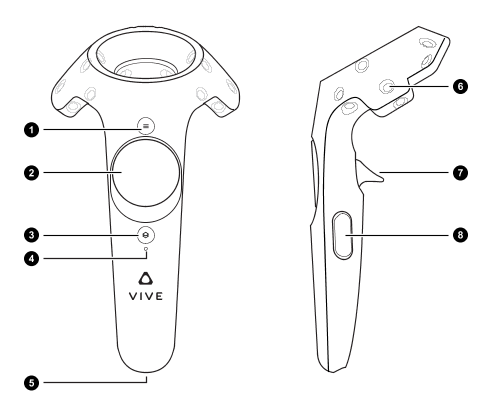
\includegraphics[width=0.8\linewidth]{vive_controller.png}
	\caption{  }
\end{figure} 

The player presses the trigger on the right controller to summon the falcon which will move towards the controller. When the game registers a collision between the controller and the falcon it sends out a "p" through the serial which can be received by an Arduino. 

On receiving the serial input the Arduino moves the servos to specified amount using the code below.

\section{Arduino Code}
\begin{lstlisting}
#include <Servo.h>

Servo clawServos[2];  
// creates and arrary of servos 

int pos = 0; 
String inputString = "";
boolean stringComplete = false;

void setup() {
	Serial.begin(9600);
	inputString.reserve(200);
	clawServos[0].attach(9);
	clawServos[1].attach(10);
	// attaches the servos on pin 9 and 10 to the servo object   
}

void loop() {
	if (stringComplete) {
	Serial.println(inputString);
	inputString = " ";
	stringComplete = false;
	}
}

void serialEvent() {
	while(Serial.available()) {
	char inChar = (char)Serial.read();
	inputString += inChar;
	
	if (inChar == '\n') {
		stringComplete = true;
	}
	
	if (inChar == 'p'){
		pinch();
		}
	}
}

void pinch() {
	for (pos = 0; pos <= 180; pos += 1) {
	// goes from 0 degrees to 180 degrees
	// in steps of 1 degree
	for (i = 0; i <= sizeof(clawServos); i += 1) {
			clawServos[i].write(pos);  
			// tell servo to go to position in variable 'pos'
	}
      
	delay(15);                       
	// waits 15ms for the servo to reach the position
	}
	for (pos = 180; pos >= 0; pos -= 1) { 
		// goes from 180 degrees to 0 degrees
		for (i = 0; i <= sizeof(clawServos); i += 1) {
			clawServos[i].write(pos); 
		}
		delay(15);
	}
}



\end{lstlisting}

\section{Arduino Diagram}
\begin{figure}[h]
	\includegraphics[width=1.0\linewidth]{arduino_diagram.png}
	\caption{  }
\end{figure} 
\bigskip



\bibliographystyle{ieeetr}
%\bibliography{comp230_1}
	
\end{document}
